%!TEX root = ../thesis.tex
\chapter{Introduction}
\label{chap:introduction}


The last couple of decades have shown a steady increase of the incidence for female breast cancer.
% An US based study published in March 2020 \cite{Lima2020Trends2015} has shown that the cancer incidence for women between the age of 25 to 39 has increased by 0.65\% per year.
In 1935 the incidence for breast cancer was at 16.3 diagnoses per 100.000 women whereas 38.5 per 100.000 women were diagnosed in the year 2015 \cite{Lima2020Trends2015}.
In Germany 71.600 women were diagnosed with breast cancer in the year 2013 with cases having doubled since 1970. A more fortunate development has been observed in the death rate in patients diagnosed with breast cancer. Since 1999 the mortality rate decreased by about a third in patients under 50 and was 25\% lower in patients between the age 50-69 during that 14 year period. 
% Some of the various reasons for the increased incidence are presumably the higher age at which women become pregnant for the first time, hormone based birth control as well as a change in diet and in exercise \cite{RobertKoch-Institut2016Bericht2016}.
One of the reasons that the mortality rate could be decreased is the screening program for women between the ages 50-69  introduced in the years 2005-2009. Since then the number of diagnoses of advanced tumour stages were decreased \cite{RobertKoch-Institut2016Bericht2016}.
The prognosis for the treatment of cancer depends on the stage of the cancer and how early it was discovered since with the size of the tumour the risk of spreading into other organs increases. As the mortality rate directly correlates with the tumour size and stage of the cancer, an early detection of cancerogenous tissue is one of the most effective ways to increase the survivability of patients \cite{Veronesi1985PrognosisNodes}, \cite{Welch2016Breast-CancerEffectiveness}.
% Among others some of the first symptoms of breast cancer often are changes in size or form of the breast as well as the formation of lumps within the breast  \cite{NationalInstitutesofHealthNIH-NationalCancerInstituteNCIBreastTreatment}.
The female breast consists of mainly fatty tissue and the mammary glands also known as lobules which produce milk occasionally during but mostly after pregnancy. Additionally, the ducts (see figure \ref{anatomy_breast}) are part of the breast tissue which form the transportation channels for the milk between the lobules and the nipple.
A very common type of breast cancer arises from this ductal system of the breast. The first symptom known as Ductal Carcinoma are calcification i.e. the deposition of calcium in the tissue of these glands.
This is a prestage of breast cancer known as stage 0 and is detectable by early mammography screening \cite{brestcancer_stages}.  


\begin{figure}[H]
    \centering
    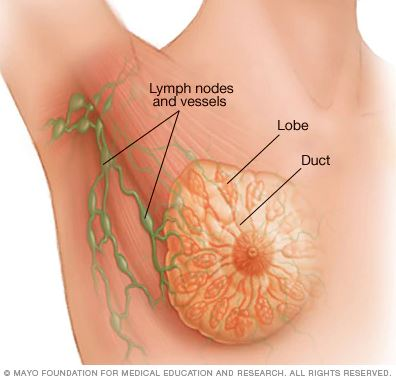
\includegraphics[width=0.65\textwidth]{Graphics/breast.jpg}
    \caption{Schematic of the female breast. The lobes form the milk producing system of the breast whereas the ducts are channels for the milk towards the nipple of the breast. Picture source: \cite{mayo-clinic}. }
    \label{anatomy_breast}
\end{figure}

\hspace{-1cm}
   
The new imaging technique \ac{usct} uses the basic principles of the ultrasound imaging technique and combines them with with the fundamental ideas of the \ac{ct}. For the measurement an ultrasound transducer emits the ultrasound wavesinto the imaging aperture of the \ac{usct}-system. The receivers record the pressure over time and yield a so called \ac{ascan}. With the combination of the \acp{ascan} yielded from the combination of all emitter-receiver-combinations an reflection and transmission image of the examined tissue can be reconstructed. The combination of multiple modalities like the reflection and attenuation for the imaging can be used to generate high resolution images with the capability to detect early stages of breast cancer. 

Compared to the widely used X-ray-based screening method which uses ionizing radiation the three dimensional \ac{usct} has its advantages and makes this novel imaging technique a promising alternative to classical mammography. By utilizing the ultrasound technique high resolution 3D images of the breast tissue can be yielded without the use of ionizing radiation. Furthermore, the examination process with an \ac{usct} is much more comfortable for the patient since the breast does not have to be deformed during the imaging procedure. 





\section{Motivation and objectives}
\label{chap:motivation}

%The characterisation of reflections of different tissue types in one major objective of this thesis.

Until now reflectivity imaging calculates the qualitative average of the reflectivity of the tissue, however the scatter characteristics of the tissue can not be characterised from these data. It can be assumed that tumour tissue consists of an inhomogeneous distribution of cancer cells which results in a distinct back scattering behaviour of this particular tissue. Similar to optical approaches it can further be assumed that small particles in the tissue have a omnidirectional reflection characteristic like a point scatterer. Tissue types with a predominant amount of inhomogeneously distribution small particles are therefore assumed to have diffuse reflection properties whereas larger, even tissue patches with homogeneous structure have a more specular reflection characteristic.
By introducing the methods for evaluating the reflection characteristic to the reconstruction algorithm, the reflection properties of different tissue types can be analysed.

Previous approaches resulted in a four dimensional image. With these four dimensions it is possible to determine a predominant direction of scattering for the tissue for each voxel in the three dimensional space. The limitations of the four dimensional approach is that the actual back scattering characteristic can not be assessed without a 2nd direction information. The 4th dimension holds the information of the voxel-receiver configuration. With the 5th dimension also the voxel-emitter relation can be regarded and used to analyse the reflection characteristics of the tissue. These limitations were tackled by extending the algorithm to a fifth dimension. Thus, not only the scalar information about the outgoing ultrasound wave from the voxel to the receiver is regarded but also the direction of the incoming pulse from the emitter to the voxel. The direction information between the fourth and fifth dimension will also allow for the analysis of reflection properties of the tissue concerning its specular and diffuse reflection parts. This leads to a specific reflection characteristic of the tissue.

The usage of platonic solids for the generation of direction vectors to discretise the directional information of the voxel in the work of Patrick Hucker \cite{PatrickHucker2014EvaluationRuckstreumodells} limited the resolution of the direction vectors and with that the capabilities to distinguish different reflection types. The generalisation of the segmentation problem of the measurement volume from small platonic solids with a limited number of directions vectors to the generation of arbitrary number of direction vectors with a higher resolution of the discretisation will increases the capabilities of the reflection analysis further. A simple example for different reflection types is given in Figure
\ref{relfec_chara_examp}:

\begin{figure}[H]
    \centering
    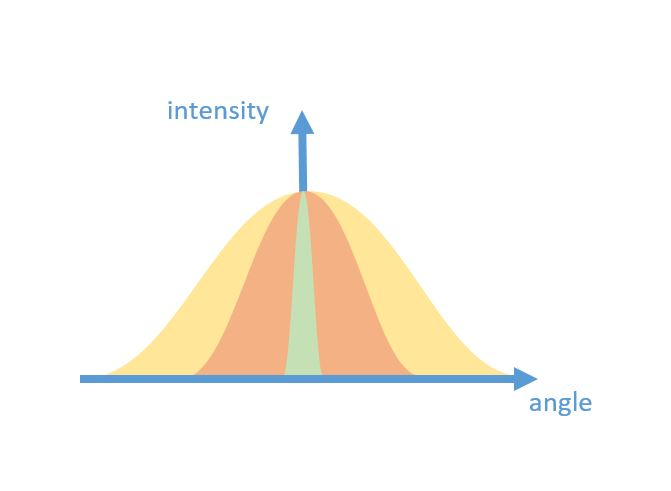
\includegraphics[width=0.56\textwidth]{Graphics/different_reflec_gauss.jpg}
    \caption{Example of three different types of reflection characteristics. The green bell curve shows close to specular reflectivity whereas the orange and yellow curves have a more diffuse reflection characteristic. }
    \label{relfec_chara_examp}
\end{figure}

To distinguish between the different reflection types it is necessary to reach a high enough discretisation of the direction information. In this thesis a new approach for the arbitrary extension of the resolution of the discretisation of the directional information is proposed, which overcomes the aforementioned limitations.

\medskip

Previous implementations for the analysis of the reflection characteristic lacked the capabilities of regarding the different \ac{sos} of tissues during the reconstruction. It was assumed that the ultrasound wave would travel with equal spread into the measurement volume. During the calculation of the \ac{sos} for the different areas of the measurement aperture the resolution of the final image could be increased. Without the \ac{sos}-correction the resolution is assumed to be insufficient to allow an distinction of the different reflection characteristics of the tissue. In this work a \ac{sos}-correction will be introduced to the reconstruction algorithm and its influence on the resulting reflection characteristics compared to non-\ac{sos}-corrected results will be assessed during this thesis.

Furthermore, the only prototypical implementation of the previous works as well as the new insights of this thesis were implemented in the production reconstruction algorithm of the \ac{usct}-project with regard to downward-compatibility and data structure.

The overall goal of this thesis is to provide insights into the reflection properties of different types of tissue and with that potentially help to further increase the clinical value of the reconstructed \ac{usct}-images in the future.

